\documentclass[12pt,a4paper,oneside]{article}

\usepackage[utf8]{inputenc}
\usepackage[portuguese]{babel}
\usepackage[T1]{fontenc}
\usepackage{amsmath}
\usepackage{amsfonts}
\usepackage{amssymb}
\usepackage{graphicx}

\usepackage{listings}
\usepackage{xcolor}

\definecolor{mygreen}{rgb}{0,0.6,0}
\definecolor{mygray}{rgb}{0.5,0.5,0.5}
\definecolor{mymauve}{rgb}{0.58,0,0.82}

\lstdefinelanguage{JavaScript}{
  keywords={typeof, new, true, false, catch, function, return, null, catch, switch, var, if, in, while, do, else, case, break},
  keywordstyle=\color{blue}\bfseries,
  ndkeywords={class, export, boolean, throw, implements, import, this},
  ndkeywordstyle=\color{darkgray}\bfseries,
  identifierstyle=\color{black},
  sensitive=false,
  comment=[l]{//},
  morecomment=[s]{/*}{*/},
  commentstyle=\color{purple}\ttfamily,
  stringstyle=\color{red}\ttfamily,
  morestring=[b]',
  morestring=[b]",
}

\lstset{ %
  backgroundcolor=\color{white},   % choose the background color; you must add \usepackage{color} or \usepackage{xcolor}
  basicstyle=\small,        % the size of the fonts that are used for the code
  breakatwhitespace=false,         % sets if automatic breaks should only happen at whitespace
  breaklines=true,                 % sets automatic line breaking
  captionpos=b,                    % sets the caption-position to bottom
  commentstyle=\color{mygreen},    % comment style
  deletekeywords={...},            % if you want to delete keywords from the given language
  escapeinside={\%*}{*)},          % if you want to add LaTeX within your code
  extendedchars=true,              % lets you use non-ASCII characters; for 8-bits encodings only, does not work with UTF-8
  frame=single,	                   % adds a frame around the code
  keepspaces=true,                 % keeps spaces in text, useful for keeping indentation of code (possibly needs columns=flexible)
  keywordstyle=\color{blue},       % keyword style
  language=HTML,                 % the language of the code
  otherkeywords={*,...},           % if you want to add more keywords to the set
  numbers=left,                    % where to put the line-numbers; possible values are (none, left, right)
  numbersep=5pt,                   % how far the line-numbers are from the code
  numberstyle=\tiny\color{mygray}, % the style that is used for the line-numbers
  rulecolor=\color{black},         % if not set, the frame-color may be changed on line-breaks within not-black text (e.g. comments (green here))
  showspaces=false,                % show spaces everywhere adding particular underscores; it overrides 'showstringspaces'
  showstringspaces=false,          % underline spaces within strings only
  showtabs=false,                  % show tabs within strings adding particular underscores
  stepnumber=1,                    % the step between two line-numbers. If it's 1, each line will be numbered
  stringstyle=\color{mymauve},     % string literal style
  tabsize=2,	                   % sets default tabsize to 2 spaces
  title=\lstname,                   % show the filename of files included with \lstinputlisting; also try caption instead of title
  moredelim=**[is][\color{purple}]{@}{@},
}

\author{\\Universidade Federal de Goiás - UFG (Regional Jataí) \\Bacharelado em Ciência da Computação \\Física para Ciência da Computação \\Prof. Esdras Lins Bispo Jr.}

\title{
	{\sc \huge Lista de Exercícios 3} 
	\\{\tt Versão 1.1}
}

\begin{document}

\maketitle

\begin{enumerate}

\section{Conceitos}
	
	\item {\bf (Halliday 2.31)} Suponha que uma nave espacial se move com uma aceleração constante de $9,8$ m/s$^2$ , o que dá aos tripulantes a ilusão de uma gravidade normal durante o voo. 
		\begin{enumerate}
			\item Se a nave parte do repouso, quanto
			tempo leva para atingir um décimo da velocidade da luz, que é $3,0 \times 10^8$  m/s?
			\item Que distância a nave percorre nesse tempo?
		\end{enumerate}
	
	\item {\bf (Halliday 2.44)} Um tatu assustado pula verticalmente para cima, subindo $0,544$ m nos primeiros $0,200$ s. 
		\begin{enumerate}
			\item Qual é a velocidade do animal ao deixar o solo?
			\item Qual é a velocidade na altura de $0,544$ m?
			\item Qual é a altura do salto?
		\end{enumerate}	
	
	\item {\bf (Halliday 2.67)} Quando uma bola de futebol é chutada na direção de um jogador e o jogador a desvia de cabeça, a aceleração da cabeça durante a colisão pode ser relativamente grande. A Figura 1 mostra a aceleração $a(t)$ da cabeça de um jogador de futebol sem e com capacete, a partir do repouso. A escala vertical é definida por $a =
	200$ m/s$^2$. Qual é a diferença entre a velocidade da cabeça sem e com o capacete no instante $t = 7,0$ ms?
		\begin{figure}
			\begin{center}
				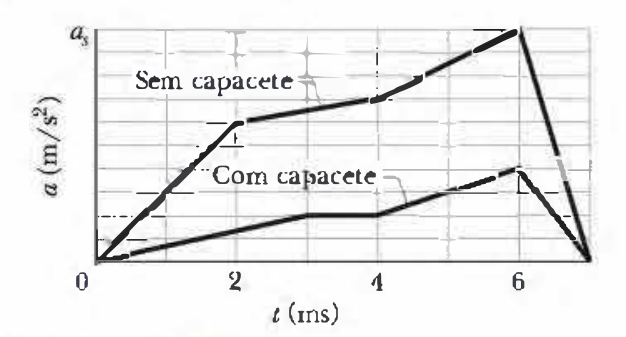
\includegraphics[scale=0.7]{imagens/grafico}
			\end{center}
			\caption{Gráfico da aceleração (m/s$^2$) pelo tempo (ms) do movimento da cabeça.}
		\end{figure}
		

\section{Programação}

	\item Em JavaScript, reescreva a função {\tt emCadaPassoX}, conforme vista em sala de aula, de forma que a bola azul ao chegar no limite direito do {\tt canvas}, ela volte na mesma direção, i.e., ela fará um movimento uniforme (MU) desta vez com a velocidade negativa. Garanta que os MUs de ida e volta permaneçam indefinidamente.
	
	\item Em JavaScript, reescreva a função {\tt emCadaPassoX}, conforme vista em sala de aula, de forma que existam duas bolas: uma bola azul e uma bola vermelha. A bola azul saindo do ponto (100, 100) e a bola vermelha saindo do ponto (600,100). A bola azul fará um movimento uniforme (MU) em direção à bola vermelha (e vice-versa). No instante anterior que as duas bolas irão colidir, é necessário garantir que ambas irão parar.
		
\end{enumerate}

\section{Referências}

\begin{itemize}
	\item HALLIDAY, D.; RESNICK, R.. Fundamentos de Física. Volume 1, Mecânica. 8ª Edição, LTC, Rio de Janeiro, 2011.

	\item RAMTAL, D.; DOBRE, A. Physics for JavaScript Games, Animation, and Simulations with HTML5 Canvas, Apress, 2014.
\end{itemize}

\end{document}